\documentclass[a4paper, 10.5pt]{ctexart}

% !!!重要提示!!! 请使用 XeLaTeX 编译此文件以获得最佳字体和排版效果。

% --- 导包 Preamble ---
% 1. 页面布局 Layout
% 调整页边距，优化空间利用率
\usepackage[left=1.4cm, right=1.4cm, top=1.8cm, bottom=2cm]{geometry}
\usepackage{graphicx}
\usepackage{xcolor}

% 2. 字体与排版 Typography
\usepackage{fontspec}
\usepackage{enumitem}
\usepackage[explicit]{titlesec}
\usepackage{microtype} % 引入 microtype 以优化微观排版和对齐

% 3. 功能增强 Utilities
\usepackage{fontawesome5}
\usepackage{hyperref}

% --- 颜色定义 Colors ---
% 定义主色调和描述文字颜色
\definecolor{PrimaryColor}{HTML}{003366} % 深海蓝，专业稳重
\definecolor{DescriptionGray}{HTML}{444444} % 优化灰度，提高可读性

% --- 字体设置 Fonts (XeLaTeX) ---
% 设置中英文字体，并提供鲁棒的备用选项
% 提升中文 AutoFakeBold 到 2.0，以在缺少粗体字重时获得更明显的加粗对比

% 中文（优先使用 方正新书宋简体 → 思源宋体 CN → macOS 自带 Songti SC）
\IfFontExistsTF{方正新书宋简体}{
  \setCJKmainfont[AutoFakeBold=2.0]{方正新书宋简体}
  \message{^^J INFO: Using Founder New Song (方正新书宋简体).^^J}
}{
  \IfFontExistsTF{思源宋体 CN}{
      \setCJKmainfont[AutoFakeBold=2.0]{思源宋体 CN}
      \message{^^J INFO: Using Source Han Serif (思源宋体 CN).^^J}
  }{
      % 最终备用（macOS 自带，命名为 Songti SC）
      \setCJKmainfont[AutoFakeBold=2.0]{Songti SC}
      \message{^^J WARNING: Preferred CJK fonts not found, falling back to Songti SC.^^J}
  }
}

% 英文（指定为 CMU Serif；无衬线优先 CMU Sans Serif，不在则回退 Helvetica Neue）
\IfFontExistsTF{CMU Serif}{
  \setmainfont{CMU Serif}
  % 无衬线：若存在 CMU Sans Serif 则使用，否则回退到 Helvetica Neue
  \IfFontExistsTF{CMU Sans Serif}{
    \setsansfont{CMU Sans Serif}
  }{
    \setsansfont{Helvetica Neue}
    \message{^^J WARNING: CMU Sans Serif not found, using Helvetica Neue as sans-serif.^^J}
  }
}{
  \setmainfont{Times New Roman}
  \setsansfont{Helvetica Neue}
  \message{^^J WARNING: CMU Serif not found, falling back to Times New Roman / Helvetica Neue.^^J}
}

% --- 设置与自定义 Configuration ---

% 超链接样式 (使用主色调)
\hypersetup{
  colorlinks=true,
  linkcolor=PrimaryColor,
  urlcolor=PrimaryColor,
  citecolor=PrimaryColor,
  pdfborder={0 0 0},
}

% 全局设置
\pagestyle{empty}
\setlength{\parindent}{0pt} % 无首行缩进
\setlength{\parskip}{0.5em} % 段落间距

% 列表紧凑设置
\setlist{itemsep=0.3em, parsep=0pt, topsep=0.5em, leftmargin=1.5em}

% --- 标题样式重定义 Section Styling ---
\titleformat{\section}
  {\normalfont\large\bfseries\color{PrimaryColor}}
  {}
  {0em}
  {#1}
  [\vspace{0.2ex}\hrule height 0.8pt]
\titlespacing*{\section}{0pt}{1.8ex}{0.8ex}

% --- 自定义命令 Commands ---
% 工作经历条目
\newcommand{\experienceEntry}[4]{%
  \noindent\textbf{#1} @ \textrm{#2} \hfill {\color{DescriptionGray}\small #3}\\
  \vspace{0.2em}%
  \begingroup
  \color{DescriptionGray}#4
  \endgroup
  \vspace{0.8em}%
}

% 中栏“经验”字号（可自定义）
% 默认与正文一致；如需自定义大小，请在导言区添加：
% \renewcommand{\ExperienceSize}{\fontsize{11pt}{13pt}\selectfont}
% 或使用 \large / \small 等字号命令：
% \renewcommand{\ExperienceSize}{\large}
\newcommand{\ExperienceSize}{10pt}
\renewcommand{\ExperienceSize}{\fontsize{10.5pt}{10.5pt}\selectfont}

\begin{document}

% --- 抬头 Header：姓名独占一行 + 下方三栏（基本信息 | 经验 | 照片） ---
\begin{center}
  {\fontsize{22pt}{24pt}\selectfont\bfseries\color{PrimaryColor} 王司晨 (Sichen Wang)}
\end{center}
\vspace{-0.3em}
\begin{tabular*}{\textwidth}{@{}p{0.45\textwidth}
  p{0\textwidth}
  p{0.20\textwidth}
  @ {\extracolsep{\fill}} p{0.20\textwidth}@{}}
  % 左列：基本信息（左对齐）
  \begin{minipage}[t]{\linewidth}
    \vspace{0pt}% 对齐三栏顶部
    {\color{DescriptionGray}
    \begin{minipage}{0.96\textwidth}
    \raggedright
    \begin{tabular}{@{}ll}
      %\faIcon{map-marker-alt} 深圳 &
      \faIcon{graduation-cap}\ 电子与计算机工程(ECE) &
      \faIcon{calendar-alt}\ 本科二年级
    \end{tabular}\\[0.2em]
    \begin{tabular}{@{}l}
      \faIcon{award}\ 专业课均分 96.0，均绩 \textbf{4.00}/4.00，一等奖学金
    \end{tabular}\\[0.2em]
    \begin{tabular}{@{}ll}
       \faIcon{phone} +86 19118814609 & 
       \faIcon{envelope} \href{mailto:sichenwang@cuhk.edu.cn}{sichenwang@cuhk.edu.cn}
    \end{tabular}
    \end{minipage}}
  \end{minipage}
  &
  % 短竖线列（固定高度）
  \begin{minipage}[t]{\linewidth}
    \vspace{0pt}\centering
    {\color{DescriptionGray}\rule{0.5pt}{2.0cm}}
  \end{minipage}
  &
  % 中列：纵向经验信息
  \begin{minipage}[t]{\linewidth}
    \vspace{0pt}% 对齐三栏顶部
    {\ExperienceSize\color{DescriptionGray}
    \begin{tabular}{@{}l @ {\hspace{0.4em}·\ } r@{}}
      \faIcon{trophy}\ 算法竞赛经验 & 8 年 \\
      \faIcon{microscope}\ 大模型科研经验 & 2 年 \\
      \faIcon{code}\ C++ 开发经验 & 9 年 \\
      \faIcon{python}\ Python 开发经验 & 3 年 \\
    \end{tabular}}
  \end{minipage}
  &
  % 右列：头像
  \begin{minipage}[t]{\linewidth}
    \vspace{-5.5em}% 对齐三栏顶部
    \begin{flushright}
      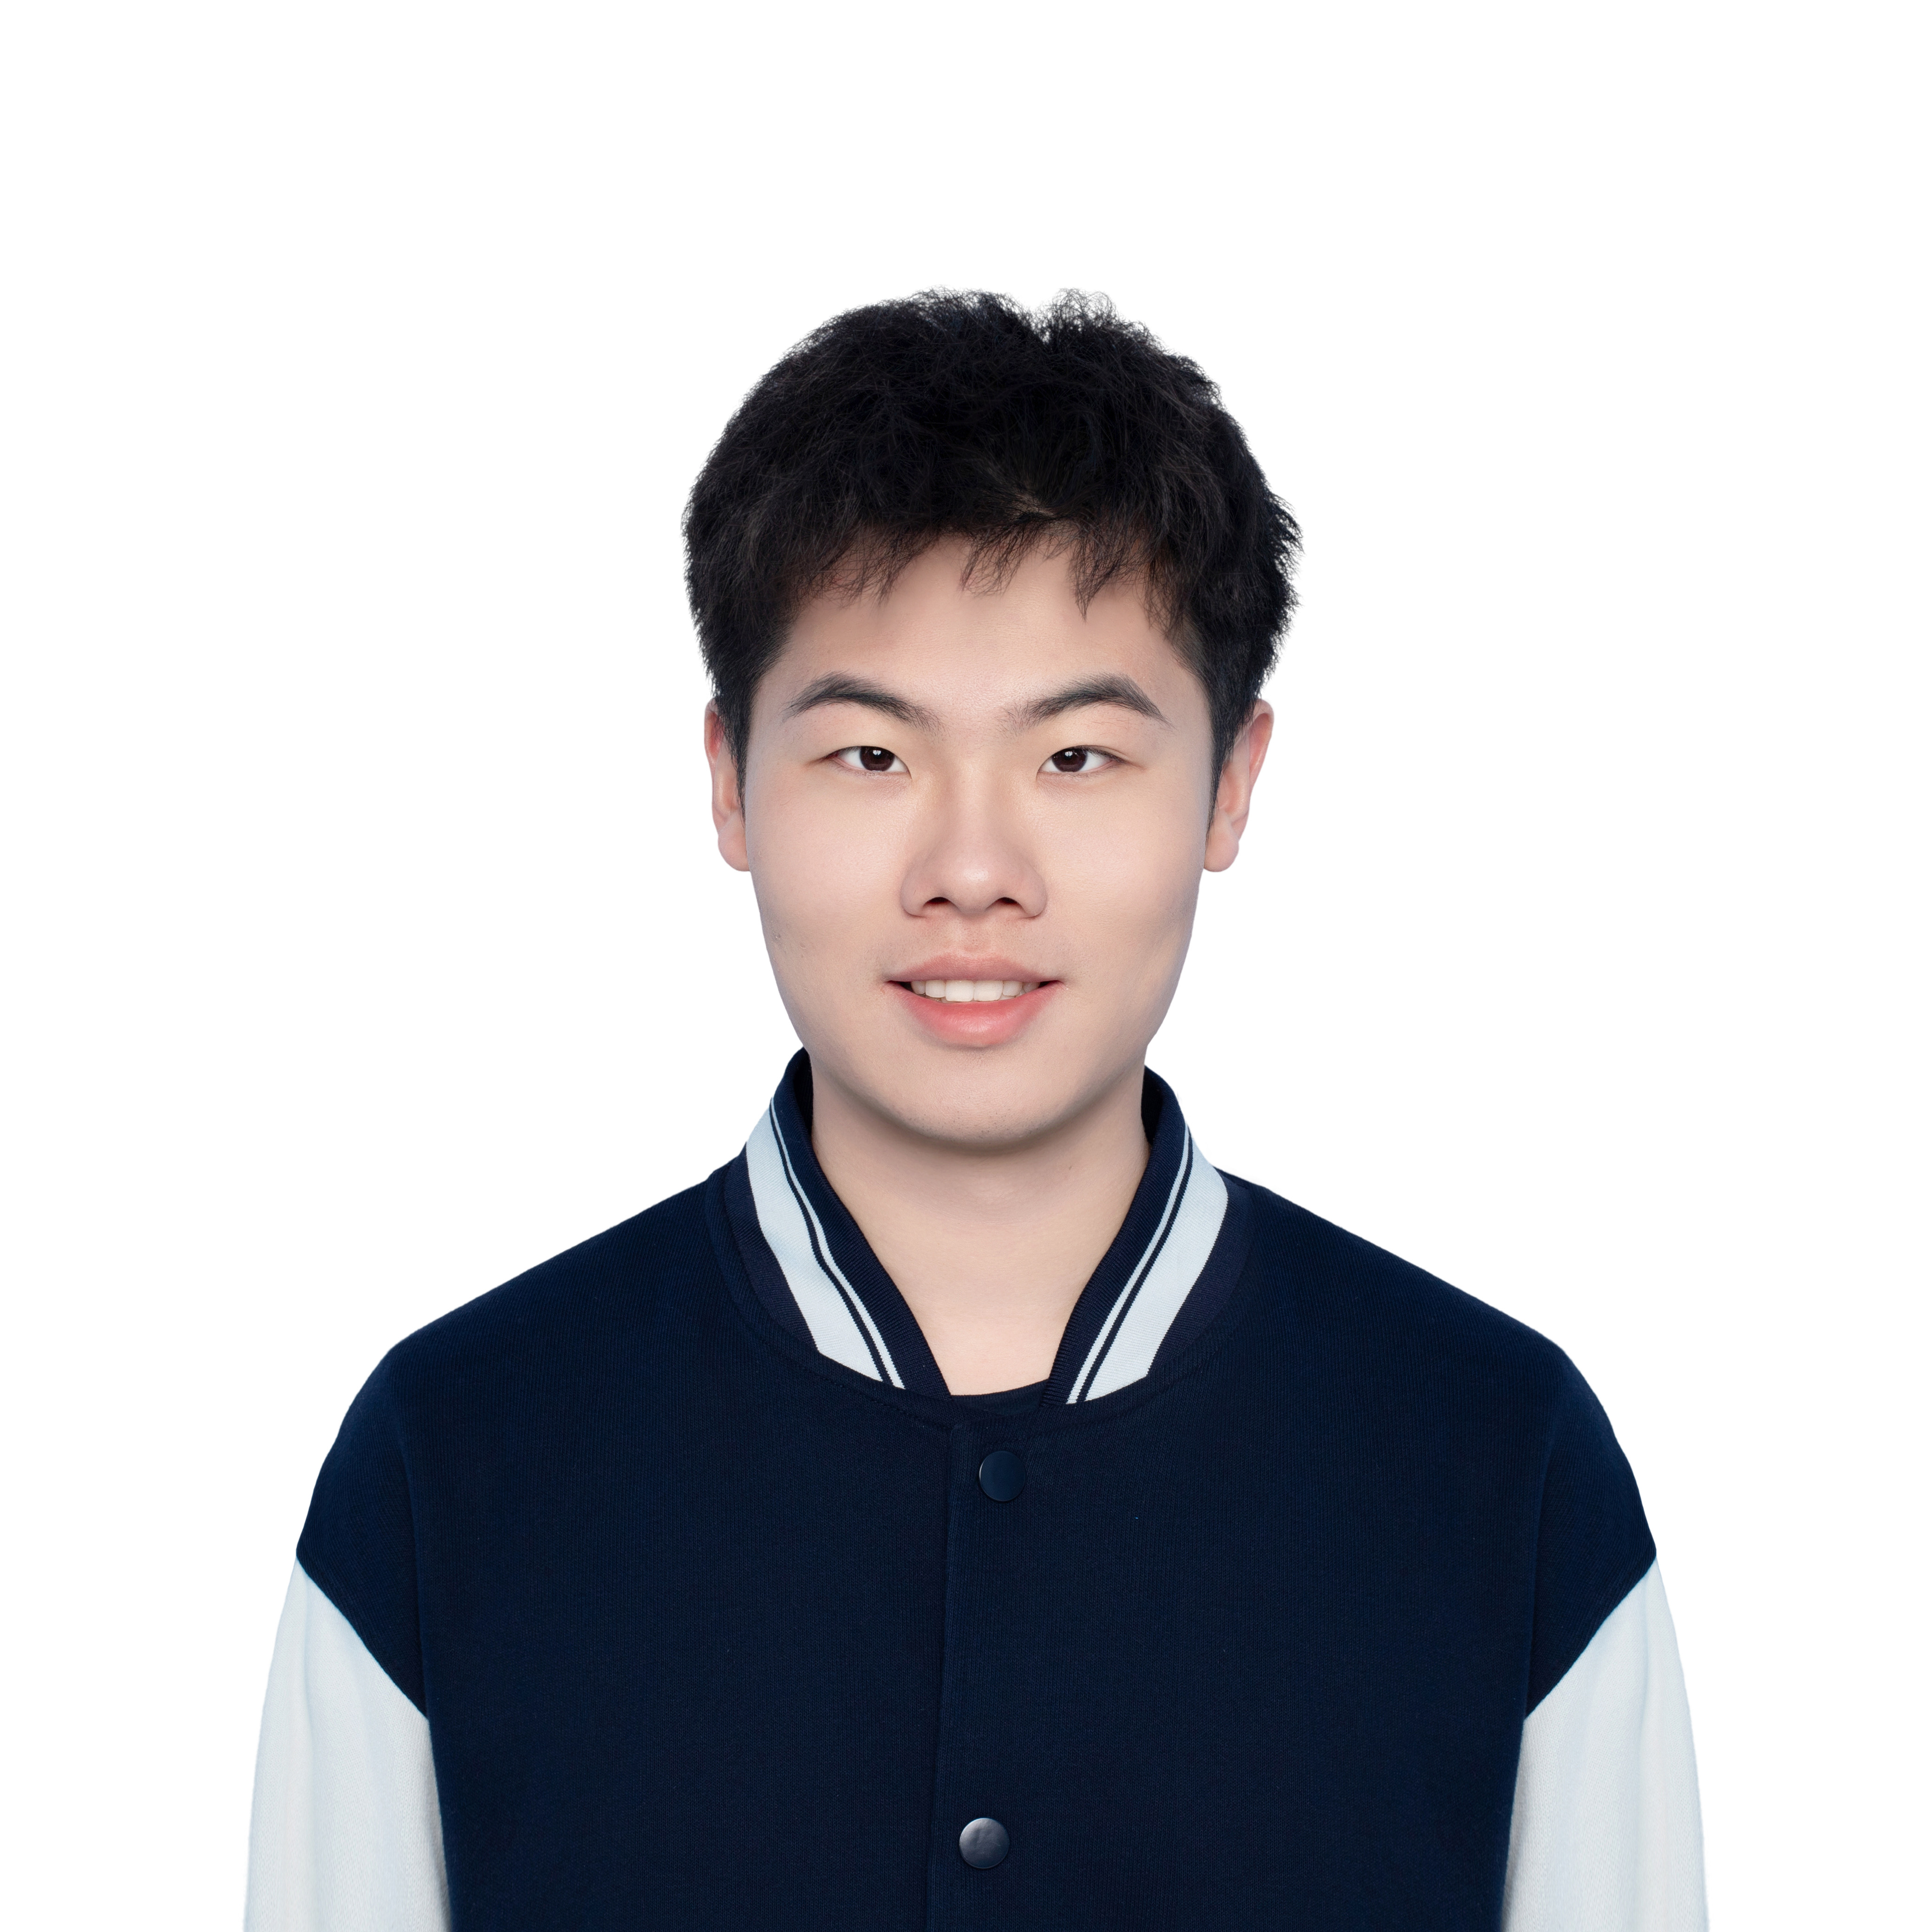
\includegraphics[height=3.8cm, keepaspectratio]{photo.JPG}
    \end{flushright}
  \end{minipage}
\end{tabular*}

\vspace{0.3em}

% --- 单栏布局开始 ---

% 研究兴趣
\section{研究兴趣 (Research Interests)}
\vspace{-0.8em}
\begin{tabular*}{\textwidth}{@{}p{0.40\textwidth} @ {\extracolsep{\fill}} p{0.505\textwidth}@{}}
  % 左列：传统方向（逐行）
  \begin{minipage}[t]{\linewidth}
    \color{DescriptionGray}
    算法设计 (Algorithm Design)\\
    理论计算机 (Theoretical Computer Science)\\
    图论 (Graph Theory)\\
    组合数学 (Combinatorics)\\
    博弈论 (Game Theory)
  \end{minipage}
  &
  % 右列：AI 方向（先列两项，再附说明）
  \begin{minipage}[t]{\linewidth}
    \color{DescriptionGray}
    AI 推理 (AI Reasoning)\\
    机器证明 (Machine Proving)\\% [0.4em]
    目前跟随香港中文大学(深圳)的唐晓莹教授进行大模型基础领域的前沿研究。
    
    正在进行的研究为 LLM Prompt Optimization 相关。
  \end{minipage}
\end{tabular*}
\color{black}

% 竞赛获奖（赛事 | 奖项 | Top x%）
\section{竞赛获奖 (Awards)}
\begin{tabular*}{\linewidth}{@{}l @{\extracolsep{\fill}} l r@{}}
  NOI 2022 冬令营 & \textbf{银牌} & \\
  连续3年 CSP-S/NOIp & \textbf{一等奖} & \\
  2024 ICPC 亚洲区域赛 (昆明站) & \textbf{金牌} & Top 3\% \\
  2024 ICPC 亚洲区域赛 (沈阳站) & \textbf{金牌} & Top 4\% \\
  2024 CCPC 中国大学生程序设计竞赛 & \textbf{金牌} & Top 4\% \\
  2024 ICPC 亚洲总决赛 (EC-Final) & \textbf{rk. 31} & Top 11\% \\
  CCPC 全国邀请赛 (广州) 个人赛 & \textbf{金牌} & Top 2\% \\
  CCF CSP 计算机软件能力认证 & \textbf{480分} & Top 0.1\% \\
  AdventureX 2025 Vibe Coding 赛道 & \textbf{冠军} & Top 1 \\
  AdventureX 2025 中控赛道 & \textbf{亚军} & Top 2 \\
\end{tabular*}

  （AdvX 参赛项目为「完全由 Multi-Agent 协同调度的自动化智能工厂架构」，全部工作 72 小时内在赛场上完成）

% 工作与实践经历
\section{工作与实践经历 (Experience)}
\experienceEntry{算法研究员}{增广智能}{}{%
独立完成论文「Data Transmission Scheduling on Grid Graph」，提出创新的「转向势能避让方法」，为公司解决了一类复杂的平面网格图上的数据调度问题。}

\experienceEntry{算法竞赛教练}{深北莫附中}{}{%
被深圳北理莫斯科大学附属中学校长特聘为信息组竞赛教练，承担高水平算法课程的讲授工作。}

\experienceEntry{算法竞赛讲师}{中国计算机学会 (CCF)}{}{%
在 2023 年大湾区青少年信息学夏令营中，负责讲课和课后答疑，并在结营考试后进行试题讲解与分析。}

\experienceEntry{算法竞赛出题人}{牛客竞赛 (Nowcoder)}{}{%
六次受邀作为牛客竞赛 (\href{https://ac.nowcoder.com}{ac.nowcoder.com}) 的出题人，承担场均 2000 人比赛的出题和讲题工作。具体包含 CSP--S 模拟赛 1 场，NOIp 模拟赛 1 场，练习赛 2 场，挑战赛 2 场。}

% 其他
% \section{其他爱好与活动 (Misc.)}
% \begin{itemize}[itemsep=0.5em, leftmargin=1.2em]
%   \item 运动: 羽毛球 (校赛八强), 网球, 乒乓球。体测 50 米 6.4 秒 (校第一)。
%   \item 音乐: 声乐, 架子鼓 (中国音协 10 级优等), 钢琴, 小提琴。
%   \item 文学: 辩论 (高中校赛冠军; 大学校赛亚军及最佳辩手), 作诗, 写散文。
% \end{itemize}

\end{document}